\documentclass[dvipdfmx]{beamer}
\usetheme[secheader]{Boadilla}
% \usepackage{beamerthemesplit} // Activate for custom appearance
%フラットデザイン化
\usefonttheme[onlymath]{serif} %数式をゴシックにしない
\setbeamertemplate{blocks}[rounded] % Blockの影を消す
\useinnertheme{circles} % 箇条書きをシンプルに
\setbeamertemplate{navigation symbols}{} % ナビゲーションシンボルを消す
\setbeamertemplate{footline}[frame number] % フッターはスライド番号のみ
\setbeamercolor{page number in head/foot}{fg=black}
% \usepackage{beamerthemesplit} // Activate for custom appearance
\setlength{\parindent}{1em}  %段落字下げ
\usepackage{tikz}
\usetikzlibrary{decorations.pathreplacing}
\usetikzlibrary{shapes, positioning,arrows,automata,arrows.meta}

\renewcommand*{\thefootnote}{\fnsymbol{footnote}}

\title{区間打切りデータに基づく情報量規準と\\感染症の潜伏期間推定への応用}
\date{2020年5月31日}
\author{神戸薬科大学  阿部興}

\begin{document}
\frame{
\titlepage
}
\section{背景}
\frame{
\frametitle{背景}
\begin{itemize}
\item 感染症の潜伏期間の分布は, 防疫上の様々な施策の基礎となる情報
\item  発症した時点が特定される場合でも, 感染した日時が観測されることはまれ
\item Backer \textit{et al.} (2020) はこの問題に対する1つのアプローチを提示
\item 新型コロナウイルス(COVID-19)感染症は最初, 中国の武漢で発生
\item  Backer \textit{et al.} (2020) は武漢への旅行者らが武漢に滞在した期間と, 発症した日のデータを用いて, 感染した時点をある種の潜在変数として扱い, 潜伏期間の分布を推定する方法を提案
\item その上で, leave-one-out (loo) 情報量規準を用いて, ワイブル分布, ガンマ分布, 対数正規分布を比較し, COVID-19感染症の潜伏期間に対してワイブル分布がよく適合すると論じた
\end{itemize}
}
\frame{
\frametitle{本報告の内容}
\begin{itemize}
\item Backer \textit{et al.} (2020) の方法論は生存時間分析の分野で区間打切り(interval censored)とよばれる観測を扱う問題と等価 
\item  Backer \textit{et al.} (2020) の用いた方法では, loo 情報量がモデルの汎化誤差の近似としてバイアスを持ち, モデル選択の方法として妥当性が十分でないことをシミュレーションを用いて示す
\item COVID-19感染症の潜伏期間は, Backer \textit{et al.}(2020) が推定したものよりも長い可能性
\end{itemize}
}
\section{観測モデルと尤度関数}
\frame{
\frametitle{データ}
\begin{itemize}
\item 2020年1月20日から28日の報告
\item 88症例
\item COVID-19感染症の患者の武漢への滞在履歴と, 発症した日が記録
\item  感染した日は未知 
\item 武漢への滞在をリスク因子への暴露とみなす
\end{itemize}

\begin{figure}[htbp]
\centering
\begin{tikzpicture}
\draw[line width=0.35mm] (0.5,0) -- (10.5,0);
\draw[line width=0.35mm] (7.0,0.25) -- (7.0,-0.25) node[above right=10pt]{発症};
\node[fill=black,draw=black,circle,inner sep=2pt,label=below:{暴露開始}] at (1,0) {};
\node[fill=white,draw=black,circle,inner sep=2pt,label=below:{感染 $s_i$}] at (3.5,0) {};
\node[fill=black,draw=black,circle,inner sep=2pt,label=below:{暴露終了}] at (6.0,0) {};
\draw [thick,decorate,decoration={brace,amplitude=6pt,raise=0pt}] (1,0.75) -- (5.9,0.75)  node [above left=8pt] {暴露の期間 $u_i$};
\draw [thick,decorate,decoration={brace,amplitude=6pt,raise=0pt}] (6.0,0.75) -- (7.0,0.75);
\node [label=above:{$t_i$}] at (6.5,1){};
\end{tikzpicture}
\caption{本報告で扱う観測}
\label{concept}
\end{figure}
}
\frame{
\frametitle{記法}

\begin{itemize}
\item 患者 $i$ が発症した日: 原点 0
\item 原点からさかのぼり, 暴露が終了した日を $t_i$ 日前とする.
\item 暴露の終了から $s_i$ 日前を感染した日とする. 
\item 暴露していた期間を $u_i$ とする.
\end{itemize}

\begin{figure}[htbp]
\centering
\begin{tikzpicture}
\draw[line width=0.35mm] (0.5,0) -- (10.5,0);
\draw[line width=0.35mm] (7.0,0.25) -- (7.0,-0.25) node[above right=10pt]{発症};
\node[fill=black,draw=black,circle,inner sep=2pt,label=below:{暴露開始}] at (1,0) {};
\node[fill=white,draw=black,circle,inner sep=2pt,label=below:{感染 $s_i$}] at (3.5,0) {};
\node[fill=black,draw=black,circle,inner sep=2pt,label=below:{暴露終了}] at (6.0,0) {};
\draw [thick,decorate,decoration={brace,amplitude=6pt,raise=0pt}] (1,0.75) -- (5.9,0.75)  node [above left=8pt] {暴露の期間 $u_i$};
\draw [thick,decorate,decoration={brace,amplitude=6pt,raise=0pt}] (6.0,0.75) -- (7.0,0.75);
\node [label=above:{$t_i$}] at (6.5,1){};
\end{tikzpicture}
\caption{本報告で扱う観測}
\label{concept}
\end{figure}
}
\frame{
\frametitle{ Backer \textit{et al.} (2020) の用いた方法}

仮に感染した時点 $s_i$ についての完全な観測が得られた場合,  発症までの待ち時間の確率密度は $f(s_i + t_i)$.  ここで $f(x)$ は確率密度関数.

\begin{itemize}
\item 尤度 
\begin{align*}
L = \prod_{i=1}^{n} f(s_i + t_i)
\end{align*}
\item 事前分布
\begin{align*}
s_i \sim \operatorname{Uniform}(0,u_i)
\end{align*}
\end{itemize}

Backer \textit{et al.} (2020) は, 確率密度関数 $f(x)$ にワイブル分布, ガンマ分布, および対数正規分布を選び, $s_i$ に区間 $[0, u_i]$ の一様事前分布を採用することで, $f(x)$ のパラメータと $s_i$ をあわせて推定. 

これを\structure{Backer 型推定}と呼ぶことにする. 
}
\frame{
\frametitle{$s_i$ を積分消去する場合}

感染した時点$s_i$を尤度から積分消去する方法も考えられる(この方法を \structure{Turnbull 型推定}と呼ぶことにする).

$s_i$ を積分消去する場合,  尤度を構成する因子の患者 $i$ に関する部分は:
\begin{align*}
\int_0 ^{u_i} f(s_i+t_i) \,ds_i.
\end{align*}
$x_i = s_i + t_i$ と改めておくと:
\begin{align*}
 \int_{t_i} ^{u_i+t_i} f(x_i) \,dx_i 
 \end{align*}
これは Turnbull (1976) が論じた区間打切りデータに基づく尤度と同じ. 
}
\frame{
\frametitle{3種類の異なる観測}
(1)-(3)式をすべてかけあわせたものが尤度関数.
\begin{enumerate}
\item $u_i= 0$ のとき, 尤度を構成する因子 $L_i$ は:
\begin{align}
L_i = f(t_i).
\end{align}
\item  $u_i$ が有限の正の実数のとき, 尤度を構成する因子 $L_i$ は:
\begin{align}
L_i = F(u_i+t_i) - F(t_i).
\end{align}
\item $u_i$ が不明のとき, 尤度を構成する因子 $L_i$ は:
\begin{align}
L_i = 1 - F(t_i).
\end{align}
\end{enumerate}
ここで $F(x)$ は $f(x)$ と対応する分布関数. 
}
\frame{
\frametitle{3種類の異なる観測}
\begin{figure}
\centering
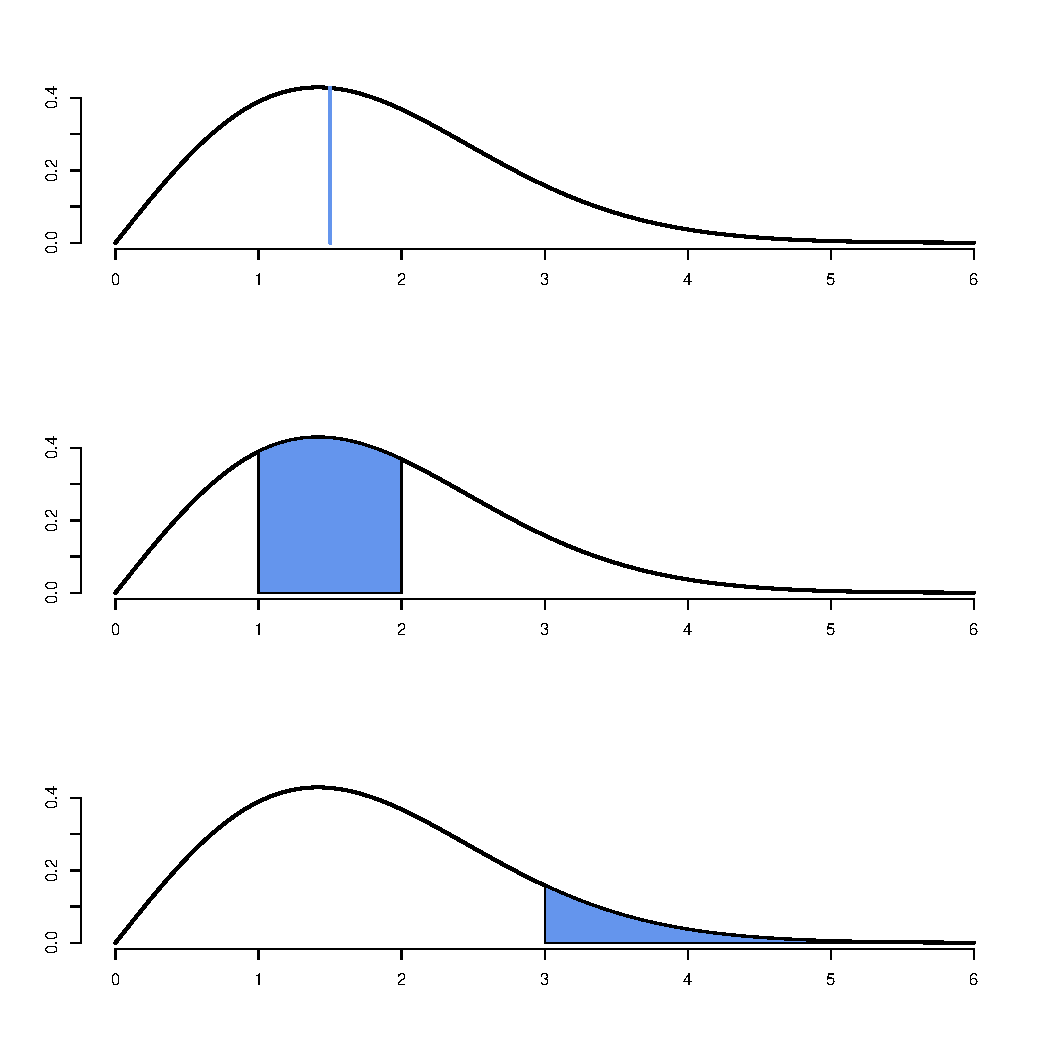
\includegraphics[width=7cm]{like3.pdf}
\caption{3種類の観測}
\end{figure}
}
\frame{
\frametitle{注意}

第3の観測($u_i$ が不明)の場合を Backer 型推定では扱うことができない. 

Backer \textit{et al.} (2020)では $u_i$ に適当な大きな数を与えることで推定を行っている. 
}

\section{情報量規準}
\frame{
\frametitle{loo 情報量}
\begin{itemize}
\item $\theta$: すべての未知パラメータ
\item $\phi(\theta)$: 事前分布の密度関数
\item $p(x|\theta)$: 評価の対象となる確率モデルの密度関数
\item $\phi^*(\theta)$: 事後分布の密度関数 
\item $\phi^*_k(\theta)$: 得られたサンプル $x_1, x_2, \ldots, x_n$ から1つのサンプル $x_k$ を\\除いてできるデータから実現された事後分布の確率密度
\end{itemize}

loo 情報量: 
\begin{align*}
\operatorname{LOOIC} =-\sum_{k=1}^n \log \left( \int p(x_k|\theta) \phi^*_k(\theta)\,d\theta. \right)
\end{align*}
}
\frame{
\frametitle{loo 情報量}
\begin{align*}
\operatorname{LOOIC} &= -\sum_{k=1}^n \log\left( 
\frac
{\int \phi(\theta)p(x_k|\theta)\prod_{i\ne k} p(x_k|\theta)\,d\theta}
{\int \phi(\theta)\prod_{i\ne k} p(x_i | \theta)\,d\theta} \right)
\\ &= -\sum_{k=1}^n  \log\left(
\frac
{\int \phi(\theta)\prod_{i=1}^n p(x_i | \theta)\,d\theta}
{\int \phi(\theta)p(x_i|\theta)^{-1}\prod_{i=1}^n p(x_i| \theta)\,d\theta}
\right)
\\ &= \sum_{k=1}^n \log\left(
\frac
{\int \phi(\theta)p(x_k|\theta)^{-1}\prod_{i=1}^n p(x_i|\theta)\,d\theta}
{\int \phi(\theta)\prod_{i=1}^n p(x_i | \theta)\,d\theta}
\right)
\\ &=\sum_{k=1}^n\log \left( \int p(x_k|\theta)^{-1} \phi^*(\theta) \, d \theta\right)
\end{align*}
サンプル1つあたりの尤度の逆数を事後分布により平均したもので, loo 情報量が計算できる. 
}
\frame{
\frametitle{汎化損失}
汎化損失:
\begin{align*}
\operatorname{GE} = -\int q(x) \log p(x) \,dx.
\end{align*}
ここで $q(x)$ はデータを生成した分布, $p(x)$ は予測分布の密度関数である.
\begin{align*}
\operatorname{GE} = \int q(x) \log \frac{q(x)}{p(x)} \,dx-\int q(x) \log q(x) \,dx.
\end{align*}
\begin{itemize}
\item 第1項: $q(x)$と$p(x)$のカルバック・ライブラ情報量
\item 第2項: データを生成した分布 $q(x)$ のみによって定まる. 予測分布 $p(x)$ の選び方に依存しない.  
\end{itemize}

汎化損失が小さいほどデータを生成した分布に近い予測分布が得られている.
}
\frame{
\frametitle{注意}
\begin{itemize}
\item loo 情報量は汎化損失の近似となる(渡辺, 2012)
\item 一般にデータを生成した分布 $q(x)$ は未知
\item 汎化損失は直接計算することができない
\item そのため, loo 情報量規準が汎化損失の近似となることが重要
\end{itemize}
}
\frame{
\frametitle{ここで生じる疑問}
サンプルごとにパラメータ(潜在変数)を持つようなモデルの場合, loo 情報量は汎化誤差の近似になるのか?

\begin{table}[ht]
\centering
\caption{leave-one-out}
\begin{tabular}{|c|c|c|}
\hline
train & train & \structure{test }\\
\hline
train & \structure{test} & train \\
\hline
 \structure{test} & train & train \\
\hline
\end{tabular}
\end{table}
}
\frame{
\frametitle{サンプル1つあたりの尤度}
 Backer 型推定とTurnbull 型推定は本質的には同じと考えられる. 
 
 しかし「サンプル1つあたりの尤度」が異なる.
 
 \vspace{\baselineskip}
 
 \begin{itemize}
 \item Backer 型推定のサンプル1つあたりの尤度:
\begin{align*}
 f(s_i + t_i)
\end{align*}
\item  Turnbull 型推定のサンプル1つあたりの尤度:
 \begin{align*}
 \int_{t_i} ^{u_i+t_i} f(x_i) \,dx_i. 
 \end{align*}
\end{itemize}
}
\section{シミュレーション}
\frame{
\frametitle{シミュレーションの設定}
Turnbull 型推定と Backer 型推定について, loo 情報量をシミュレーション.
\begin{itemize}
\item Backer \textit{et al.} (2020)に習い, すべてのパラメータの事前分布に一様分布(フラットプライヤ)を採用
\item 事後分布の実現には確率的プログラミング言語 Stan を用いた
\item データを生成する分布: ワイブル分布(形状パラメータ, 尺度パラメータともに2) 
\item 評価の対象となるモデルの確率分布: ワイブル分布
\item シミュレーションの試行回数: 100回
\item サンプルサイズ: $n = 25,  50, 100$
\item 区間打切りは生成したデータの小数点以下を切り落とすことにより\footnote{例を上げると 1.5 という乱数が生成された場合, これを区間 $[1, 2]$ の区間打切りデータとして扱う}, 人工的に生成
\end{itemize}
 }
\frame{
\frametitle{シミュレーション結果}

\begin{figure}
\centering
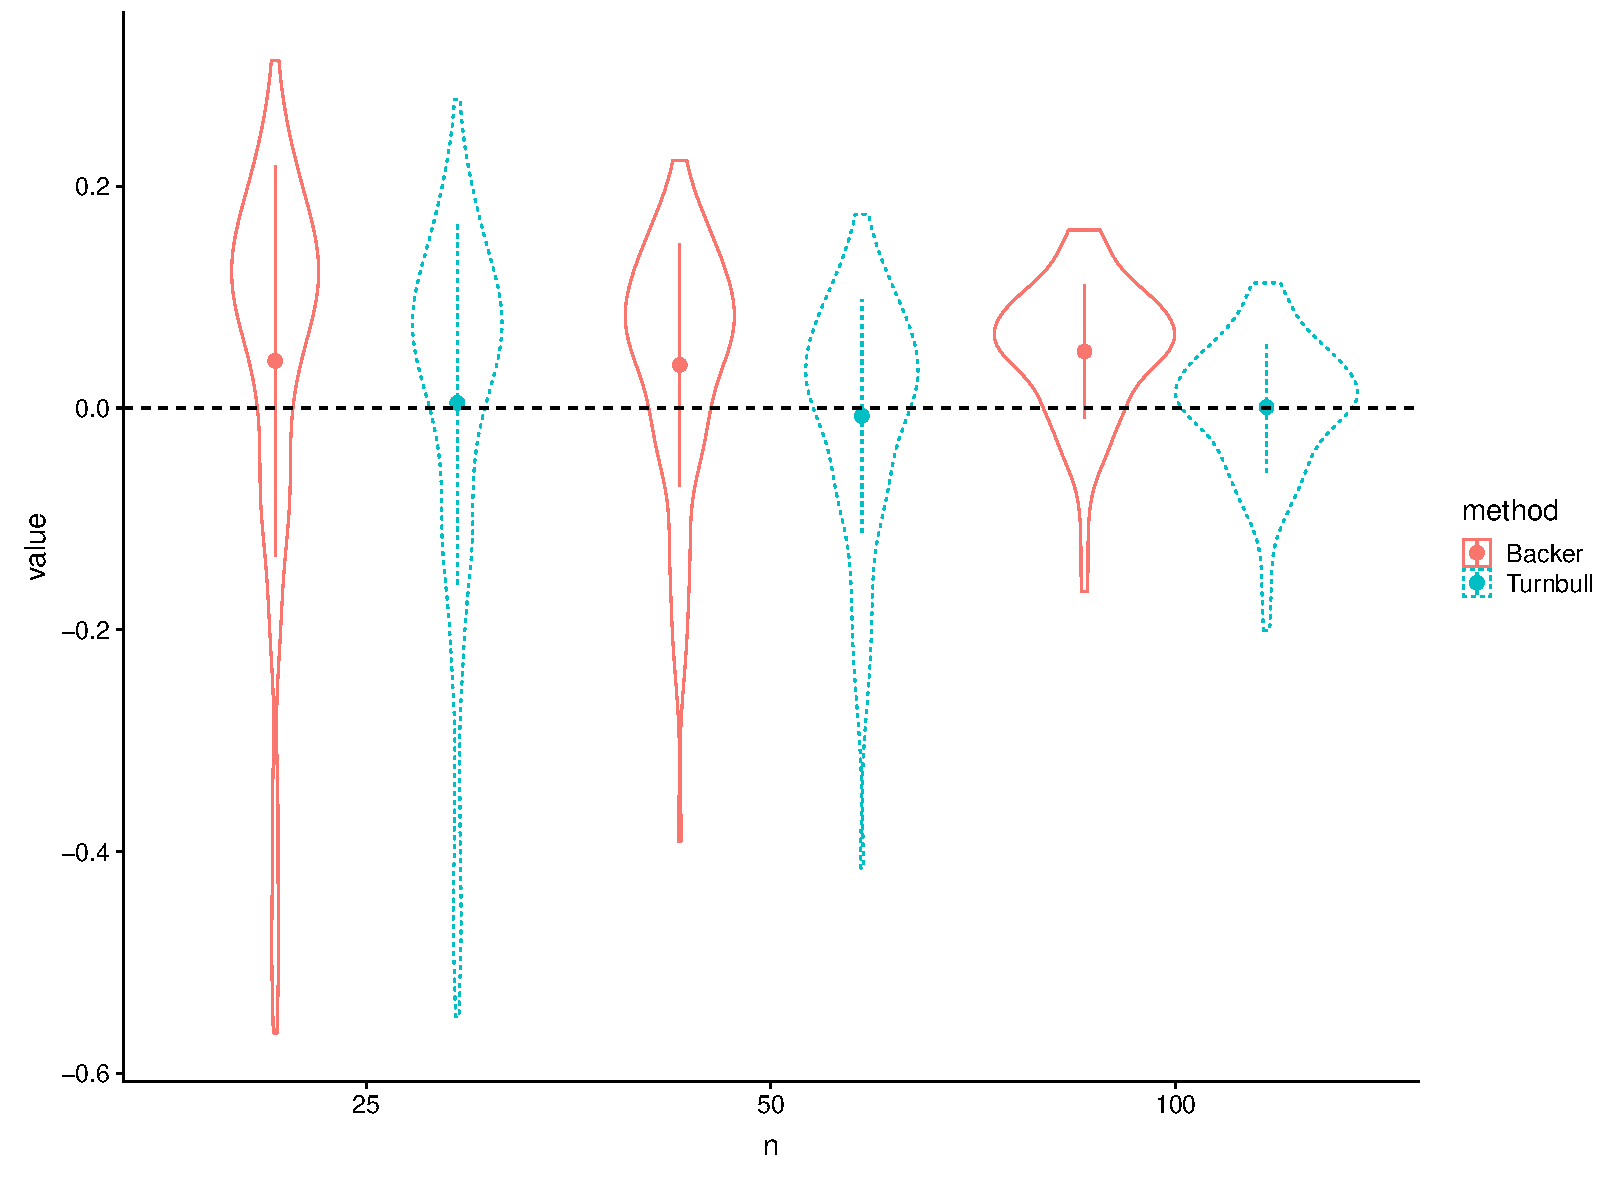
\includegraphics[width=7cm]{simGEplot.pdf}
\caption{シミュレーション結果. エラーバーは標準偏差, 点は平均を表す.}
\label{simGEplot}
\end{figure}

図中の value は $\operatorname{GE}- \operatorname{LOOIC}/n$.
}
\frame{
\frametitle{パラメータの推定量としての違い}

\begin{table}[ht]
\centering
\caption{推定量(事後期待値)の平均}
\begin{tabular}{r|rrrr}
  \hline
&\multicolumn{2}{c}{形状パラメータ} &\multicolumn{2}{c}{尺度パラメータ}\\ 
$n$ & Turnbull & Backer & Turnbull & Backer \\ 
  \hline
25 & 2.18 & 2.18 & 2.08 & 2.08 \\ 
  50 & 2.09 & 2.09 & 2.03 & 2.03 \\ 
  100 & 2.03 & 2.03 & 2.01 & 2.01 \\ 
   \hline
\end{tabular}
\end{table}

\begin{table}[ht]
\centering
\caption{推定量(事後期待値)の標準誤差}
\begin{tabular}{r|rrrr}
  \hline
&\multicolumn{2}{c}{形状パラメータ} &\multicolumn{2}{c}{尺度パラメータ}\\ 
$n$ & Turnbull & Backer & Turnbull & Backer \\ 
  \hline
25 & 0.45 & 0.45 & 0.23 & 0.23 \\ 
50 & 0.30 & 0.30 & 0.18 & 0.18 \\ 
100 & 0.20 & 0.20 & 0.12 & 0.12 \\ 
   \hline
\end{tabular}
\end{table}
}
\frame{
\frametitle{シミュレーション結果に対する考察}
\begin{itemize}
\item Backer 型推定では loo情報量は汎化損失の推定量としてバイアスを持つ
\item バイアスはサンプルサイズを大きくしても小さくならない 
\item Turnbull 型推定はより正確に汎化損失を近似
\end{itemize}
}
\section{データ分析}
\frame{
\frametitle{実データでの例}

Backer \textit{et al.} (2020) と同じデータを用いて Turnbull 型推定により loo 情報量を計算した.
 
\begin{tabular}{cc}
\begin{minipage}{0.45\textwidth}
\begin{table}[ht]
\centering
\caption{Turnbull 型推定}
\begin{tabular}{lr}
  \hline
分布 & loo情報量 \\ 
  \hline
ワイブル & 73.89 \\ 
ガンマ & 73.35 \\ 
対数正規 & 73.32 \\ 
   \hline
\end{tabular}
\end{table}
\end{minipage}
&
\begin{minipage}{0.45\textwidth}
\begin{table}[ht]
\centering
\caption{Backer \textit{et al.} (2020) より}
\begin{tabular}{lr}
  \hline
分布 & loo情報量 \\ 
  \hline
ワイブル & 486 \\ 
ガンマ & 545 \\ 
対数正規 & 592 \\ 
   \hline
\end{tabular}
\end{table}
\end{minipage}
\end{tabular}
この表でのloo情報量は $\operatorname{LOOIC}$ の2倍.
}
\frame{
\frametitle{潜伏期間の分布}

対数正規分布が最も裾の重い予測を与える.

\begin{figure}
\centering
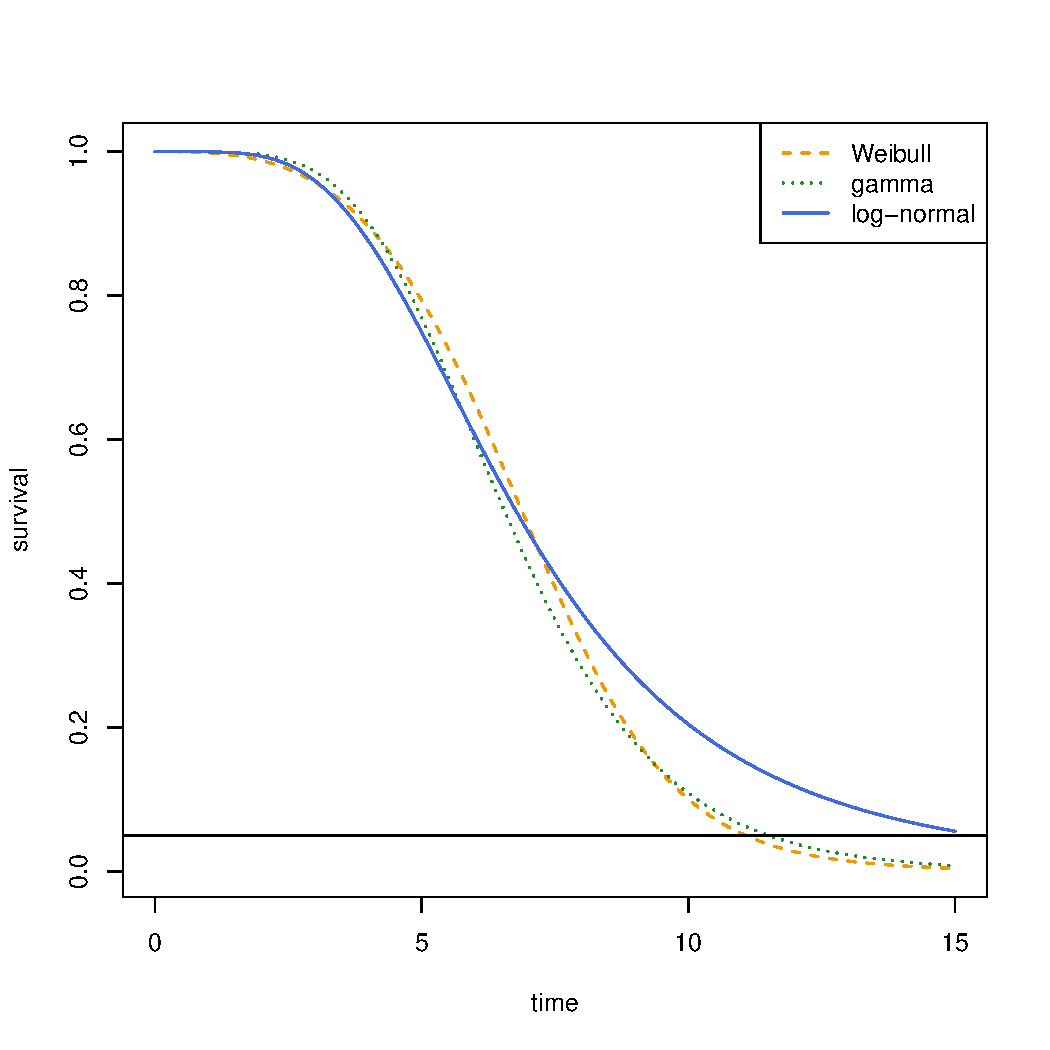
\includegraphics[width=6cm]{survfit.pdf}
\caption{潜伏期間の生存関数}
\end{figure}
}
\frame{
\frametitle{予測区間}

\begin{table}[ht]
\centering
\caption{潜伏期間の予測区間}
\begin{tabular}{rrrr}
  \hline
 & 2.5\% & 50\% & 97.5\% \\ 
  \hline
ワイブル & 2.52 & 6.86 & 12.11 \\ 
ガンマ & 2.97 & 6.55 & 12.89 \\ 
対数正規 & 2.66 & 6.78 & 18.99 \\ 
   \hline
\end{tabular}
\end{table}

\structure{参考}: Backer \textit{et al.} (2020) の示した95\%予測区間は$[2.1, 11.1]$
}
\section{まとめ}
\frame{
\frametitle{議論}
\begin{itemize}
\item 潜在変数がある場合の情報量規準の使用には注意が必要
\item COVID-19感染症の潜伏期間は, Backer \textit{et al.}(2020) の推定より長い可能性
\item 潜伏期間の情報は確立されたものではなく, さらなる議論が必要なもの
\end{itemize}
}
\frame{
\frametitle{参考文献}
\begin{itemize}
\item Backer, J. A., Klinkenberg, D., \& Wallinga, J. (2020). Incubation period of 2019 novel coronavirus (2019-nCoV) infections among travellers from Wuhan, China, 20-28 January 2020. \textit{Eurosurveillance}, 25(5), 2000062.
\item Turnbull, B. W. (1976). The empirical distribution function with arbitrarily grouped, censored and truncated data. Journal of the Royal Statistical Society: Series B (Methodological), 38(3), 290-295.
\item 渡辺澄夫 (2012). \textbf{ベイズ統計の理論と方法.} コロナ社.
%\bibitem{} Vehtari, A., Gelman, A., \& Gabry, J. (2017). Practical Bayesian model evaluation using leave-one-out cross-validation and WAIC. Statistics and computing, 27(5), 1413-1432.
\end{itemize}
}
\frame{
\frametitle{シミュレーションの設定}
Turnbull 型推定と Backer 型推定について, loo 情報量をシミュレーション.
\begin{itemize}
\item Backer \textit{et al.} (2020)に習い, すべてのパラメータの事前分布に一様分布(フラットプライヤ)を採用
\item 事後分布の実現には確率的プログラミング言語 Stan を用いた
\item データを生成する分布: ガンマ分布(形状パラメータ2, レートパラメータ0.25) 
\item 評価の対象となるモデルの確率分布: ガンマ分布
\item シミュレーションの試行回数: 100回
\item サンプルサイズ: $n = 25,  50, 100$
\item 区間打切りは生成したデータの小数点以下を切り落とすことにより, 人工的に生成
\end{itemize}
 }
\frame{
\frametitle{ガンマ分布の場合}
\begin{figure}
\centering
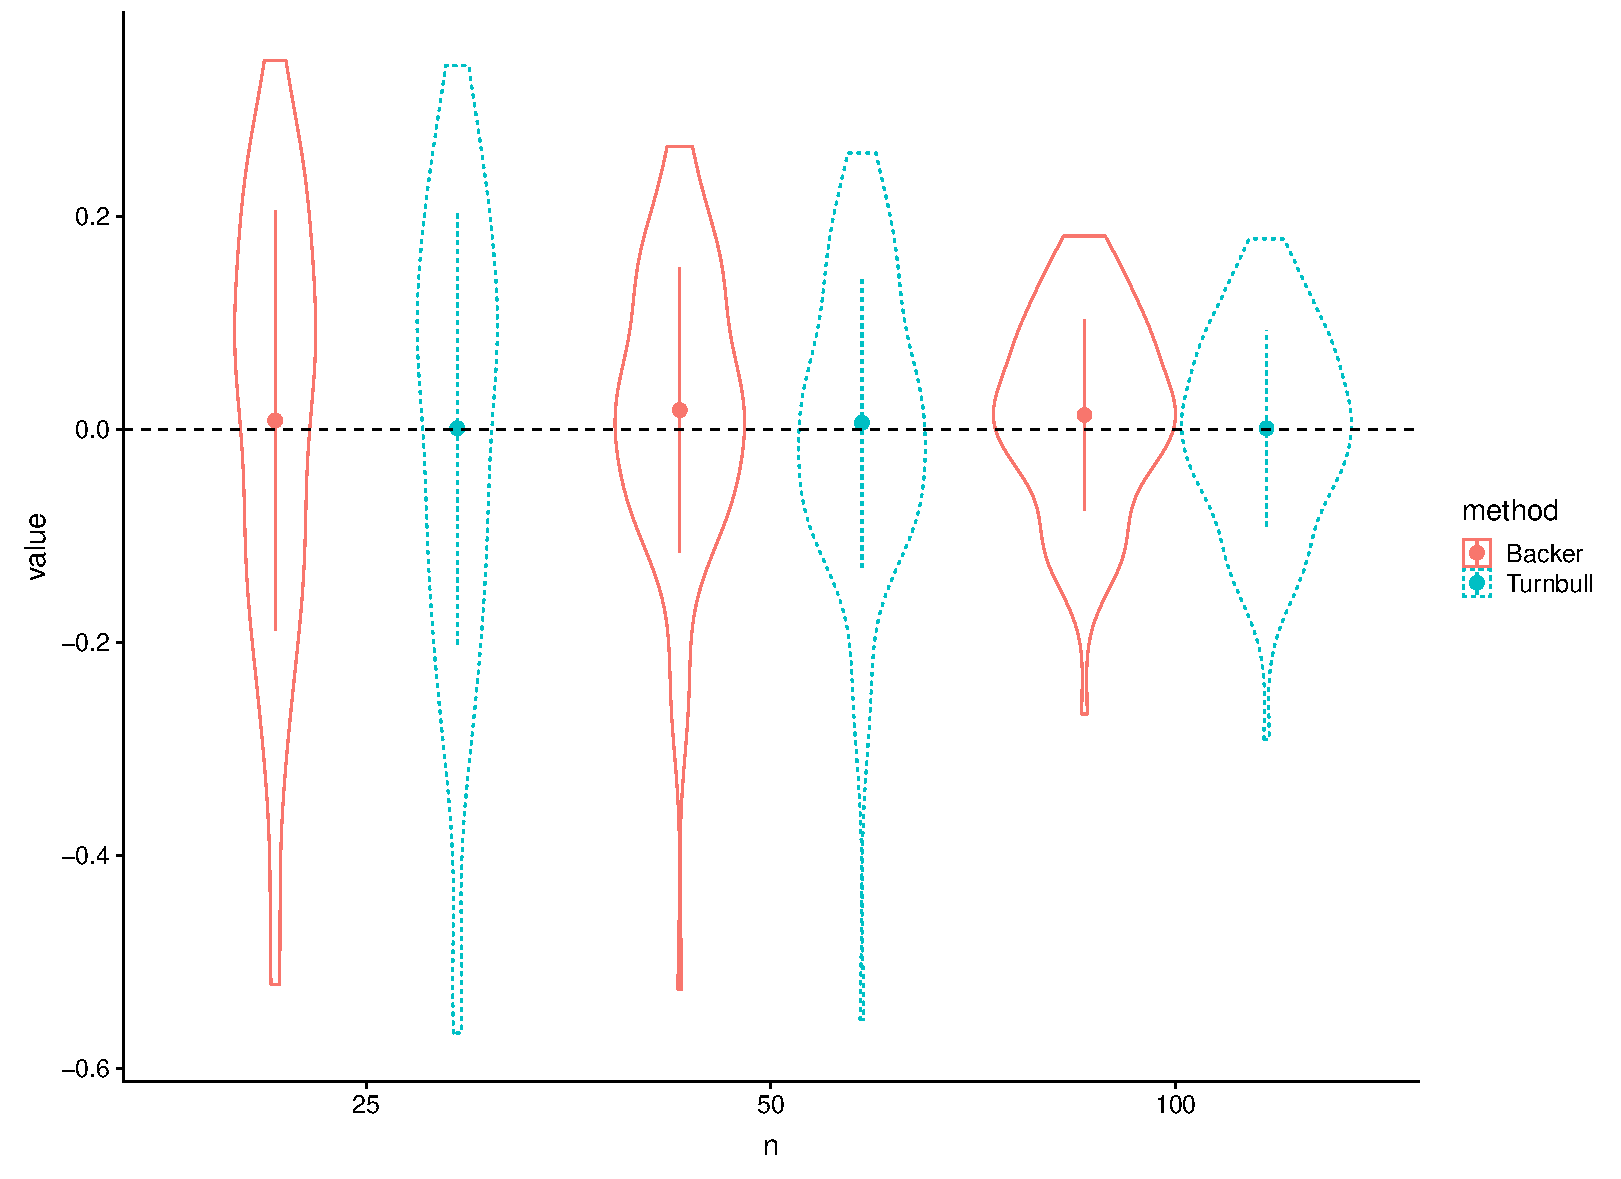
\includegraphics[width=7cm]{simGEplot_gamma.pdf}
\caption{シミュレーション結果. エラーバーは標準偏差, 点は平均を表す.}
\label{simGEplot}
\end{figure}

図中の value は $\operatorname{GE}- \operatorname{LOOIC}/n$.
}
\frame{
\frametitle{シミュレーションの設定}
Turnbull 型推定と Backer 型推定について, loo 情報量をシミュレーション.
\begin{itemize}
\item Backer \textit{et al.} (2020)に習い, すべてのパラメータの事前分布に一様分布(フラットプライヤ)を採用
\item 事後分布の実現には確率的プログラミング言語 Stan を用いた
\item データを生成する分布: 対数正規分布(平均パラメータ0, 分散パラメータ1) 
\item 評価の対象となるモデルの確率分布: 対数正規分布
\item シミュレーションの試行回数: 100回
\item サンプルサイズ: $n = 25,  50, 100$
\item 区間打切りは生成したデータの小数点以下を切り落とすことにより, 人工的に生成
\end{itemize}
 }
\frame{
\frametitle{対数正規分布の場合}
\begin{figure}
\centering
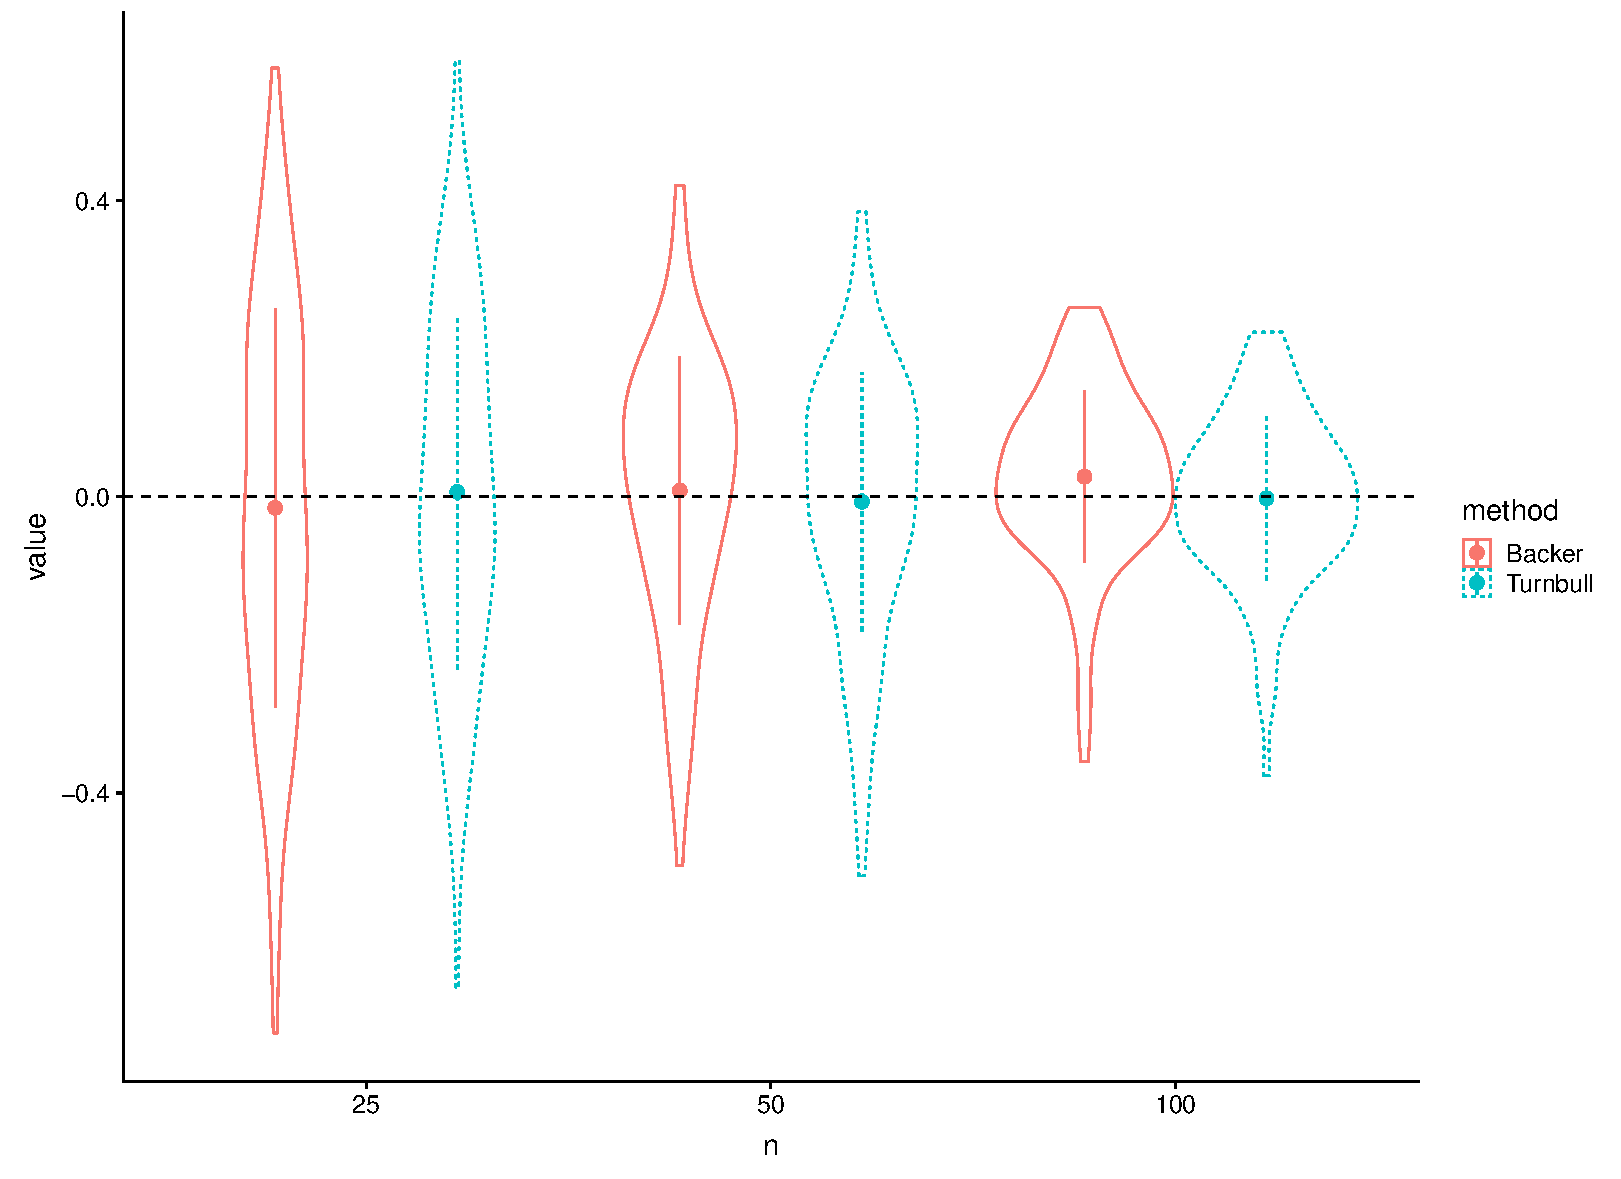
\includegraphics[width=7cm]{simGEplot_lnorm.pdf}
\caption{シミュレーション結果. エラーバーは標準偏差, 点は平均を表す.}
\label{simGEplot}
\end{figure}

図中の value は $\operatorname{GE}- \operatorname{LOOIC}/n$.
}
\end{document}  